\begin{enumerate}[label=\thechapter.\arabic*,ref=\thechapter.\theenumi]
\item Let y\brak{t}=x\brak{4t},where x\brak{t} is a continous-time periodic signal of $100$s.the fundamental period of y\brak{t} is (\textbf{rounded off to the nearest integer})
 \hfill(GATE IN 2023)\\
\solution
\iffalse
\let\negmedspace\undefined
\let\negthickspace\undefined
\documentclass[journal,12pt,twocolumn]{IEEEtran}
\usepackage{cite}
\usepackage{amsmath,amssymb,amsfonts,amsthm}
\usepackage{algorithmic}
\usepackage{graphicx}
\usepackage{textcomp}
\usepackage{xcolor}
\usepackage{txfonts}
\usepackage{listings}
\usepackage{enumitem}
\usepackage{mathtools}
\usepackage{gensymb}
\usepackage{comment}
\usepackage[breaklinks=true]{hyperref}
\usepackage{tkz-euclide} 
\usepackage{listings}
\usepackage{gvv}                                        
\def\inputGnumericTable{}                                 
\usepackage[latin1]{inputenc}                                
\usepackage{color}                                            
\usepackage{array}                                            
\usepackage{longtable}                                       
\usepackage{calc}                                             
\usepackage{multirow}                                         
\usepackage{hhline}                                           
\usepackage{ifthen}                                           
\usepackage{lscape}

\newtheorem{theorem}{Theorem}[section]
\newtheorem{problem}{Problem}
\newtheorem{proposition}{Proposition}[section]
\newtheorem{lemma}{Lemma}[section]
\newtheorem{corollary}[theorem]{Corollary}
\newtheorem{example}{Example}[section]
\newtheorem{definition}[problem]{Definition}
\newcommand{\BEQA}{\begin{eqnarray}}
\newcommand{\EEQA}{\end{eqnarray}}
\newcommand{\define}{\stackrel{\triangle}{=}}
\theoremstyle{remark}
\newtheorem{rem}{Remark}
\begin{document}

\bibliographystyle{IEEEtran}
\vspace{3cm}

\title{GATE 2023 IN 29}
\author{EE23BTECH11065 - prem sagar}
\maketitle
\newpage

\bigskip 

\renewcommand{\thefigure}{\theenumi}
\renewcommand{\thetable}{\theenumi}
\textbf{Question}:
\\\\Let y\brak{t}=x\brak{4t},where x\brak{t} is a continous-time periodic signal of $100$s.the fundamental period of y\brak{t} is (\textbf{rounded off to the nearest integer})
 \hfill(GATE IN 29)
 \\\\\textbf{Solution}:
\fi
\begin{table}[!ht]
\def\arraystretch{1.5}
   \centering
    \renewcommand\thetable{1}
      \begin{tabular}{|c|c|c|}
   \hline
   \textbf{Symbol} & \textbf{Value}& \textbf{Description} \\
   \hline
         $T$ & $100$ & fundamental period of $x\brak{t}$\\
        \hline
        $T_1$ &  & fundamental period of y\brak{t}\\
        \hline
        $\omega_0$ & $\frac{8\pi}{100} $  & fundamental frequency of y\brak{t}\\
        \hline
\end{tabular}

    \caption{input parameters}
    \label{tab:IN 29}
 \end{table}
\\From \tabref{tab:IN 29}
\\Applying Fourier series:
 \begin{align}
 x\brak{t}&=\sum_{n=-\infty}^{\infty}c_ne^\frac{j\;2\pi n\;t}{100}
\\ y\brak{t}&=x\brak{4t}
\\ y\brak{t}&=\sum_{n=-\infty}^{\infty}c_ne^\frac{j\;2\pi n\;\brak{4t}}{100}
\\&=\sum_{n=-\infty}^{\infty}c_ne^\frac{j\;2\pi n\;t}{25}
\\T_1&=25\text{sec}
 \end{align}
\begin{figure}[h]
 \renewcommand\thefigure{1}
    \centering
    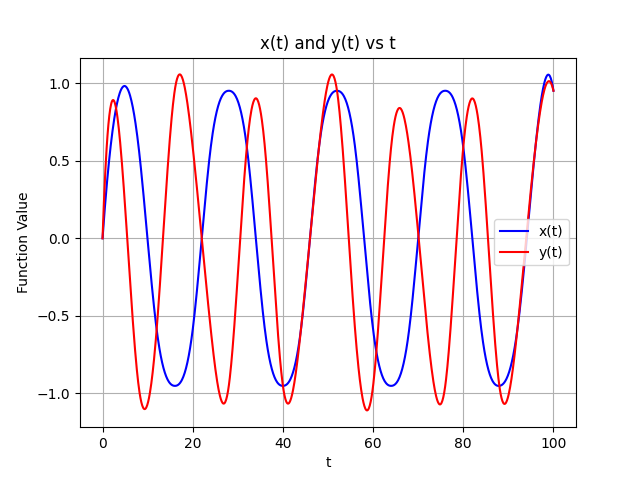
\includegraphics[width=1\linewidth]{2023/IN/29/figs/figr.png}
    \caption{plot y\brak{t} v/s t}
\end{figure}
%\end{document}

\newpage
\item In the circuit shown below, it is observed that the amplitude of voltage across the resistor is the same as the amplitude of the sorce voltage. What is the angular frequency $\omega_0$(in rad$/s$)?\\

\begin{circuitikz}[american]
    \draw (0,0) to[R, l=$10K\Omega$] (2,0) to[L, l=$10mH$] (4,0) to[C, l=$1\mu{F}$] (6,0) -- (6,-1) 
    to[sV, l=$100\cos(\omega_0 t)$] (0,-1) -- (0,0)
    (0,-1) node[circ]{} node[left]{$+$}
    (6,-1) node[circ]{} node[right]{$-$};
\end{circuitikz} \hfill(GATE BM 2023)
\solution
\newpage

\item For a regular sinusoidal wave propagating in deep water having wave height of 3.5 m and wave period of 9 s, the wave steepness is \underline{\hspace{1cm}} (round off to three decimal places).
\hfill Gate 2023 NM 33\\
\solution
\let\negmedspace\undefined
\let\negthickspace\undefined
\documentclass[journal,12pt,onecolumn]{IEEEtran}
\usepackage{cite}
\usepackage{amsmath,amssymb,amsfonts,amsthm}
\usepackage{algorithmic}
\usepackage{graphicx}
\usepackage{textcomp}
\usepackage{tikz}
\usepackage{xcolor}
\usepackage{txfonts}
\usepackage{listings}
\usepackage{enumitem}
\usepackage{mathtools}
\usepackage{gensymb}

\usepackage{tkz-euclide} % loads  TikZ and tkz-base
\usepackage{listings}



\newtheorem{theorem}{Theorem}[section]
\newtheorem{problem}{Problem}
\newtheorem{proposition}{Proposition}[section]
\newtheorem{lemma}{Lemma}[section]
\newtheorem{corollary}[theorem]{Corollary}
\newtheorem{example}{Example}[section]
\newtheorem{definition}[problem]{Definition}
%\newtheorem{thm}{Theorem}[section] 
%\newtheorem{defn}[thm]{Definition}
%\newtheorem{algorithm}{Algorithm}[section]
%\newtheorem{cor}{Corollary}
\newcommand{\BEQA}{\begin{eqnarray}}
\newcommand{\EEQA}{\end{eqnarray}}
\newcommand{\system}[1]{\stackrel{#1}{\rightarrow}}

\newcommand{\define}{\stackrel{\triangle}{=}}
\theoremstyle{remark}
\newtheorem{rem}{Remark}
%\bibliographystyle{ieeetr}
\begin{document}
%
\providecommand{\pr}[1]{\ensuremath{\Pr\left(#1\right)}}
\providecommand{\prt}[2]{\ensuremath{p_{#1}^{\left(#2\right)} }}        % own macro for this question
\providecommand{\qfunc}[1]{\ensuremath{Q\left(#1\right)}}
\providecommand{\sbrak}[1]{\ensuremath{{}\left[#1\right]}}
\providecommand{\lsbrak}[1]{\ensuremath{{}\left[#1\right.}}
\providecommand{\rsbrak}[1]{\ensuremath{{}\left.#1\right]}}
\providecommand{\brak}[1]{\ensuremath{\left(#1\right)}}
\providecommand{\lbrak}[1]{\ensuremath{\left(#1\right.}}
\providecommand{\rbrak}[1]{\ensuremath{\left.#1\right)}}
\providecommand{\cbrak}[1]{\ensuremath{\left\{#1\right\}}}
\providecommand{\lcbrak}[1]{\ensuremath{\left\{#1\right.}}
\providecommand{\rcbrak}[1]{\ensuremath{\left.#1\right\}}}
\newcommand{\sgn}{\mathop{\mathrm{sgn}}}
\providecommand{\abs}[1]{\left\vert#1\right\vert}
\providecommand{\res}[1]{\Res\displaylimits_{#1}} 
\providecommand{\norm}[1]{\left\lVert#1\right\rVert}
%\providecommand{\norm}[1]{\lVert#1\rVert}
\providecommand{\mtx}[1]{\mathbf{#1}}
\providecommand{\mean}[1]{E\left[ #1 \right]}
\providecommand{\cond}[2]{#1\middle|#2}
\providecommand{\fourier}{\overset{\mathcal{F}}{ \rightleftharpoons}}
\newenvironment{amatrix}[1]{%
  \left(\begin{array}{@{}*{#1}{c}|c@{}}
}{%
  \end{array}\right)
}
%\providecommand{\hilbert}{\overset{\mathcal{H}}{ \rightleftharpoons}}
%\providecommand{\system}{\overset{\mathcal{H}}{ \longleftrightarrow}}
	%\newcommand{\solution}[2]{\textbf{Solution:}{#1}}
\newcommand{\solution}{\noindent \textbf{Solution: }}
\newcommand{\cosec}{\,\text{cosec}\,}
\providecommand{\dec}[2]{\ensuremath{\overset{#1}{\underset{#2}{\gtrless}}}}
\newcommand{\myvec}[1]{\ensuremath{\begin{pmatrix}#1\end{pmatrix}}}
\newcommand{\mydet}[1]{\ensuremath{\begin{vmatrix}#1\end{vmatrix}}}
\newcommand{\myaugvec}[2]{\ensuremath{\begin{amatrix}{#1}#2\end{amatrix}}}
\providecommand{\rank}{\text{rank}}
\providecommand{\pr}[1]{\ensuremath{\Pr\left(#1\right)}}
\providecommand{\qfunc}[1]{\ensuremath{Q\left(#1\right)}}
	\newcommand*{\permcomb}[4][0mu]{{{}^{#3}\mkern#1#2_{#4}}}
\newcommand*{\perm}[1][-3mu]{\permcomb[#1]{P}}
\newcommand*{\comb}[1][-1mu]{\permcomb[#1]{C}}
\providecommand{\qfunc}[1]{\ensuremath{Q\left(#1\right)}}
\providecommand{\gauss}[2]{\mathcal{N}\ensuremath{\left(#1,#2\right)}}
\providecommand{\diff}[2]{\ensuremath{\frac{d{#1}}{d{#2}}}}
\providecommand{\myceil}[1]{\left \lceil #1 \right \rceil }
\newcommand\figref{Fig.~\ref}
\newcommand\tabref{Table~\ref}
\newcommand{\sinc}{\,\text{sinc}\,}
\newcommand{\rect}{\,\text{rect}\,}
%%
%	%\newcommand{\solution}[2]{\textbf{Solution:}{#1}}
%\newcommand{\solution}{\noindent \textbf{Solution: }}
%\newcommand{\cosec}{\,\text{cosec}\,}
%\numberwithin{equation}{section}
%\numberwithin{equation}{subsection}
%\numberwithin{problem}{section}
%\numberwithin{definition}{section}
%\makeatletter
%\@addtoreset{figure}{problem}
%\makeatother

%\let\StandardTheFigure\thefigure
\let\vec\mathbf

\bibliographystyle{IEEEtran}





\bigskip


\title{Gate 2023\_nm\_33}
\author{Karyampudi Meghana Sai\\ EE23BTECH11031}

\maketitle

For a regular sinusoidal wave propagating in deep water having wave height of 3.5 m and wave period of 9 s, the wave steepness is \underline{\hspace{1cm}} (round off to three decimal places).
\hfill Gate 2023 NM 33

\solution

\begin{table}[h]
 	\centering
 	\resizebox{6 cm}{!}{
 		\begin{tabular}{|c|c|c|}
	\hline
	\textbf{Symbol} & \textbf{Value} &
	\textbf{Description}\\[6pt]
	\hline
	$H$ &  $3.5m$ & wave height\\[6pt]
	\hline 
	$T$ & $9s$ & wave period\\[6pt]
	\hline
	$S$ & $ ? $ & wave steepness\\[6pt]
	\hline
	$\lambda$ & $  $ & wave length\\[6pt]
	\hline
	$\eta$ & $  $ & surface elevation of water\\[6pt]
	\hline
\end{tabular}

 	}
 	\vspace{6 pt}
 	\caption{Input Parameters}
 	\label{table:gatenm33table1} 
 \end{table} 
 
 \begin{figure}[h!]
    \centering
    \resizebox{0.55\columnwidth}{!}{\documentclass{standalone}
\usepackage{tikz}

\begin{document}

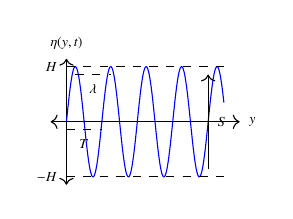
\begin{tikzpicture}[x=0.2cm, y=0.2cm,font=\tiny] % Adjusted scaling for smaller plot
    % Draw axes
    \draw[<->] (-1,0) -- (11,0) node[right] {$y$}; % Adjusted x-axis length
    \draw[<->] (0,-4) -- (0,4) node[above] {$\eta(y,t)$}; % Adjusted y-axis length
    % Draw wave
    \draw[blue, thin, domain=0:10, smooth,samples=900] plot (\x, {3.5*sin(8*pi*\x/9 r)});
    % Draw wave height
    \draw[dashed] (0,3.5) node[left] {$H$} -- (10,3.5) ; % Adjusted x-axis length
    \draw[dashed] (0,-3.5) node[left] {$-H$} -- (10,-3.5) ; % Adjusted x-axis length
    % Draw wave period
    \draw[dashed] (0,-0.5) -- (2.25,-0.5) node[midway, below] {$T$}; % Adjusted x-axis range
    
    % Draw wavelength
    \draw[dashed] (0.5625,3) -- (2.8125,3) node[midway, below] {$\lambda$}; % Adjusted x-axis range
    % Draw wave steepness
    \draw[->] (9,-3) -- (9,3) node[midway,right] {$S$}; % Adjusted x-axis range
\end{tikzpicture}

\end{document}

}
    \caption{Sinusoidal wave}
    \label{fig:gatenm33fig1}
\end{figure} 


\begin{enumerate}
 \item Deriving the formula for wavelength of deep water wave:\\
\begin{align}
S&=\frac{H}{\lambda} \label{eq:gatenm33eq1}
\end{align}
Let's start with the linearized shallow water wave equation.\\
\begin{align}
\frac{\partial^2 \eta}{\partial t^2}=g \frac{\partial \eta}{\partial y}\label{eq:gatenm33eq2}\\
\eta = A\sin(ky - \omega t) \label{eq:gatenm33eq3} \\
\frac{\partial^2 \eta}{\partial t^2} = -(\omega)^2 A\sin(ky - \omega t) \label{eq:gatenm33eq4}
\end{align}
For deep water waves:\\ 
\begin{align}
\frac{\partial \eta}{\partial y} &\approx -k\eta \label{eq:gatenm33eq5}
\end{align}
Using the equation \eqref{eq:gatenm33eq2}.
\begin{align}
\frac{\partial^2 \eta}{\partial t^2}&=-gk\eta \label{eq:gatenm33eq6}\\
&=-gk A\sin(ky - \omega t) \label{eq:gatenm33eq7}
\end{align}
where, k is wave number. \\

Comparing equations \eqref{eq:gatenm33eq4} and \eqref{eq:gatenm33eq7},\\
\begin{align}
\omega^2 &= gk \label{eq:gatenm33eq8} \\
\omega &= \frac{2 \pi}{T} \label{eq:gatenm33eq9} \\
k &= \frac{2 \pi}{\lambda} \label{eq:gatenm33eq10} \\
\lambda &= \frac{g \cdot T^2}{2 \pi} \label{eq:gatenm33eq11}
\end{align}
\item Numerical computation:\\
\begin{align}
\lambda&=\frac{g \cdot T^2}{2\pi}\\ 
&=\frac{9.81 \brak{9}^2}{2\pi}\\ 
&=126.53m 
\end{align}
Using the equation \eqref{eq:gatenm33eq1}.\\
\begin{align}
S&=\frac{3.5}{126.53}\\ 
&=0.028 
\end{align}
\end{enumerate}
\begin{figure}[h]
    \centering
    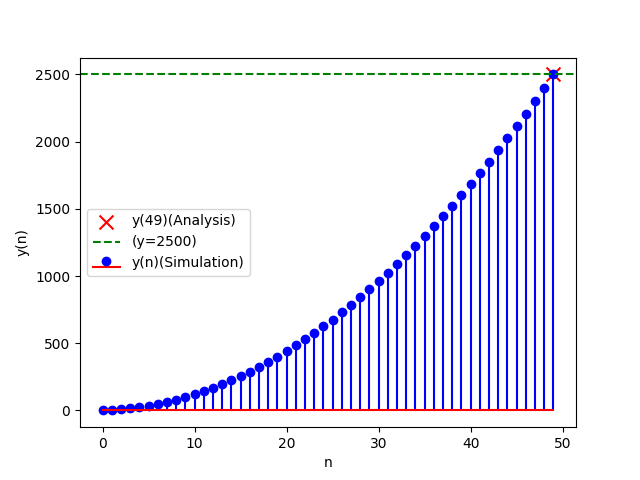
\includegraphics[width=\columnwidth]{figs/plot.png}
    \caption{Sinusoidal wave}
    \label{fig:gatenm33fig2}
\end{figure} 

\end{document}



\newpage

\item  A spring mass system is shown in the figure . Take the value of acceleration  due to gravity as $g=9.81m/s^2$.The static deflection due to weight and the time period of the oscillations,respectively,are\\
 \begin{figure}[h!]
    \centering
    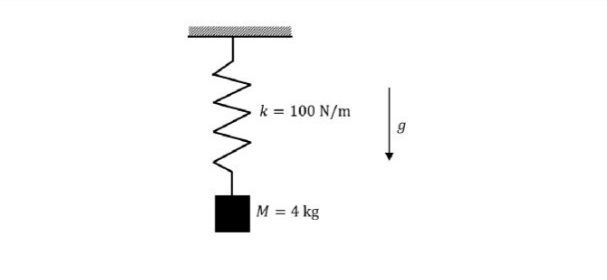
\includegraphics[width = \columnwidth]{2023/XE/71/figs/fig1.jpg}
\end{figure}
\hfill{(GATE 2023 XE)}\\
\solution
\iffalse
\let\negmedspace\undefined
\let\negthickspace\undefined
\documentclass[journal,12pt,twocolumn]{IEEEtran}
\usepackage{cite}
\usepackage{amsmath,amssymb,amsfonts,amsthm}
\usepackage{algorithmic}
\usepackage{graphicx}
\usepackage{textcomp}
\usepackage{xcolor}
\usepackage{txfonts}
\usepackage{listings}
\usepackage{enumitem}
\usepackage{mathtools}
\usepackage{gensymb}
\usepackage{comment}
\usepackage[breaklinks=true]{hyperref}
\usepackage{tkz-euclide} 
\usepackage{listings}
\usepackage{gvv}                                        
\def\inputGnumericTable{}                                 
\usepackage[latin1]{inputenc}                                
\usepackage{color}                                            
\usepackage{array}                                            
\usepackage{longtable}                                       
\usepackage{calc}                                             
\usepackage{multirow}                                         
\usepackage{hhline}                                           
\usepackage{ifthen}                                           
\usepackage{lscape}

\newtheorem{theorem}{Theorem}[section]
\newtheorem{problem}{Problem}
\newtheorem{proposition}{Proposition}[section]
\newtheorem{lemma}{Lemma}[section]
\newtheorem{corollary}[theorem]{Corollary}
\newtheorem{example}{Example}[section]
\newtheorem{definition}[problem]{Definition}
\newcommand{\BEQA}{\begin{eqnarray}}
 \newcommand{\EEQA}{\end{eqnarray}}
\newcommand{\define}{\stackrel{\triangle}{=}}
\theoremstyle{remark}
\newtheorem{rem}{Remark}
\begin{document}
 \bibliographystyle{IEEEtran}
 \vspace{3cm}
 \title{\textbf{XE 71}}
 \author{EE23BTECH11048-Ponugumati Venkata Chanakya$^{*}$% <-this % stops a space
 }
 \maketitle
 \newpage
 \bigskip
 \renewcommand{\thefigure}{\theenumi}
 \renewcommand{\thetable}{\theenumi}
 \textbf{QUESTION:}
 A spring mass system is shown in the figure . Take the value of acceleration  due to gravity as $g=9.81m/s^2$.The static deflection due to weight and the time period of the oscillations,respectively,are\\
 \begin{figure}[h!]
    \centering
    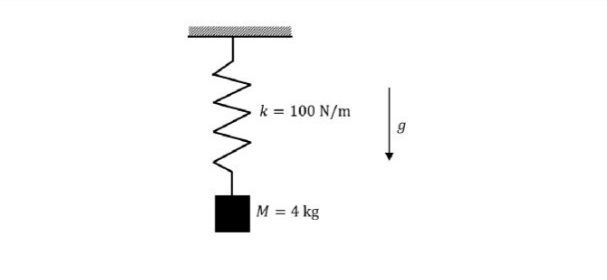
\includegraphics[width = \columnwidth]{2023/XE/71/figs/xe_71_f1.png}
\end{figure}
\hfill{(GATE2023 XE)}\\
\solution
\fi
\begin{enumerate}
    \item Static deflection due to weight(sdw)\\
    let x be sdw.\\0
    At mean position in equilibrium\\
    \ref{XE_71.t1}
    \begin{align}
        Mg&=kx\\
        x&=39.24cm
    \end{align}
     \item Time period of oscillation\\
     \begin{align}
           F&=-kx\\
           m\brak{\frac{d^2x}{dt^2}}&=-kx
     \end{align}
      Initial Conditions be at extreme  point of SHM
      \begin{align}
       x(0)&=0.3924 \label{XE_71.5}\\
       \frac{dx}{dt}&=0 \text{ at } t=0 \text{ (released from rest)} \label{XE_71.6}
        \end{align} 
     Taking Laplace transform:
     \begin{align}
     m(s^2X(s)-sx(0)-mx'(0))+kX(s)&=0
     \end{align}
     \begin{align}
      X(s) &= \frac{x(0)ms+mx'(0)}{ms^2 + k}\\
      X(s)&=x(0)\frac{s}{s^2+\frac{k}{m}}+\brak{x'(0)\sqrt{\frac{k}{m}}}\frac{\sqrt{\frac{k}{m}}}{s^2+\brak{\sqrt{\frac{k}{m}}}^2}
      \end{align}
     Taking Inverse Laplace Transform:\\
     \begin{align}
     x(t)&=x(0)\cos\left(\sqrt{\frac{k}{m}}t\right)+\brak{x'(0)\sqrt{\frac{k}{m}}}\sin \brak{\sqrt{\frac{k}{m}}t}\\
     \end{align}
     Using \ref{XE_71.5} and \ref{XE_71.6} 
     \begin{align}
      x(t) &= 0.3924 \cos\left(\sqrt{\frac{k}{m}}t\right)\\
      x(t)&=39.24 \sin\brak{5t+\frac{\pi}{2}} \text{ cm}
     \end{align}
    The static deflection due to weight and the time period of the oscillations,respectively are $39.24$ cm and $\frac{2\pi}{5}$ s
\end{enumerate}
 \begin{figure}[h!]
    \centering
    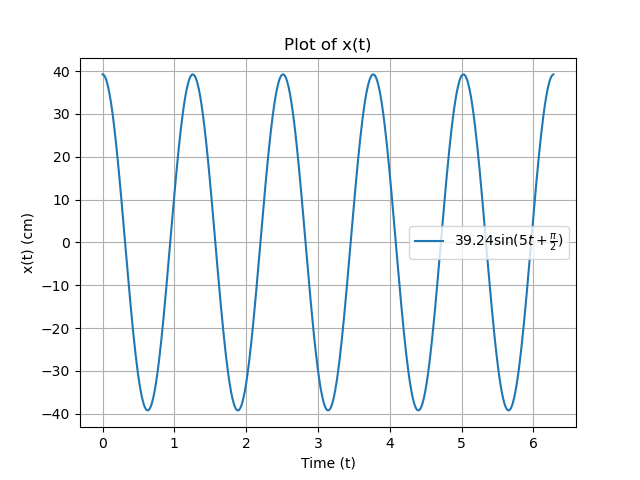
\includegraphics[width = \columnwidth]{2023/XE/71/figs/xe_71_f2.png}
\end{figure}
 \begin{table}[!ht]
    \centering
             \begin{tabular}{|c|c|c|} 
      \hline
\textbf{Variable}& \textbf{Description}& \textbf{Value}\\\hline
         $M$& weight of block &$4$ kg\\\hline
          $K$ & spring constant & $100\frac{N}{m}$  \\\hline
          $x$& Static deflection due to weight&$39.24$ cm\\\hline  
          $x(t)$& Displacement of particle from mean position at time t  & none \\\hline
          $x(0)$& Initial Displacement of particle from mean position  & $39.24$cm \\\hline
           $x'(t)$& velocity of particle & none \\\hline
          $x'(0)$& initial velocity of particle & $0$ \\\hline
    \end{tabular}

    \caption{input parameters}
     \label{XE_71.t1}
\end{table}
%\end{document}


\pagebreak

\item In the circuit shown below, the amplitudes of the voltage across the resistor and the capacitor are equal. What is the value of the angular frequency $\omega_o$ (in rad/s)? 
(Round off the answer to one decimal place.) \hfill(GATE BM 32 2023)
\begin{circuitikz}
    % Voltage source
    \draw (0,0) to[sV, v=$100\cos(\omega_{o} t)$] (0,2);
    
    % Resistor
    \draw (0,2) to[R, l=$1\text{ k}\Omega$] (3,2);
    
    % Capacitor
    \draw (3,2) to[C, l=$100\mu\text{F}$] (3,0);
    
    % Ground
    \draw (3,0) -- (0,0);
\end{circuitikz}
\solution
\iffalse
\let\negmedspace\undefined
\let\negthickspace\undefined
\documentclass[journal,12pt,twocolumn]{IEEEtran}
\usepackage{cite}
\usepackage{amsmath,amssymb,amsfonts,amsthm}
\usepackage{algorithmic}
\usepackage{graphicx}
\usepackage{textcomp}
\usepackage{xcolor}
\usepackage{txfonts}
\usepackage{listings}
\usepackage{enumitem}
\usepackage{mathtools}
\usepackage{gensymb}
\usepackage[breaklinks=true]{hyperref}
\usepackage{tkz-euclide} % loads  TikZ and tkz-base
\usepackage{listings}
\usepackage{gvv}
\usepackage{circuitikz}

\newtheorem{theorem}{Theorem}[section]
\newtheorem{problem}{Problem}
\newtheorem{proposition}{Proposition}[section]
\newtheorem{lemma}{Lemma}[section]
\newtheorem{corollary}[theorem]{Corollary}
\newtheorem{example}{Example}[section]
\newtheorem{definition}[problem]{Definition}

\newcommand{\BEQA}{\begin{eqnarray}}
\newcommand{\EEQA}{\end{eqnarray}}
\newcommand{\define}{\stackrel{\triangle}{=}}
\theoremstyle{remark}
\newtheorem{rem}{Remark}

\graphicspath{./figs/}

%\bibliographystyle{ieeetr}
\begin{document}
%

\bibliographystyle{IEEEtran}


\vspace{3cm}

\title{
	%	\logo{
	Gate Assignment

	\large{EE:1205 Signals and Systems}

	Indian Institute of Technology, Hyderabad
	%	}
}
\author{Kunal Thorawade

EE23BTECH11035
}	
\maketitle


\newpage

%\tableofcontents

\bigskip
 
 \renewcommand{\thefigure}{\theenumi}
 \renewcommand{\thetable}{\arabic{table}}
 \renewcommand{\thefigure}{\arabic{figure}}
 %\renewcommand{\theequation}{\theenumi}

 \textbf{Question}:
 In the circuit shown below, the amplitudes of the voltage across the resistor and the capacitor are equal. What is the value of the angular frequency $\omega_o$ (in rad/s)? 
 (Round off the answer to one decimal place.)
 \hfill(GATE BM 32 2023)
 \begin{circuitikz}
	     % Voltage source
	     \draw (0,0) to[sV, v=$100\cos(\omega_{0} t)$] (0,2);
	         
		     % Resistor
		         \draw (0,2) to[R, l=$1\text{ k}\Omega$] (3,2);
			     
			         % Capacitor
				     \draw (3,2) to[C, l=$100\mu\text{F}$] (3,0);
				         % Ground
					     \draw (3,0) -- (0,0);
 \end{circuitikz}

 \solution
 \fi
 \begin{table}[ht]
	  \centering
	    \begin{tabular}{|c|c|c|}
		        \hline
			   \textbf{ Parameter} & \textbf{Value} & \textbf{Description} \\
			       \hline
			           $v\brak{t}$ & $100cos\brak{\omega_0 t}$ & Input Voltage \\
				       \hline
				           $R$ & $1\text{ k}\Omega$ & Resistance \\
					       \hline
					           $C$ & $100\mu\text{F}$ & Capacitance \\
						       \hline
						           $\omega_0$ & ? & Angular Frequency  \\
							       \hline
							           $Z_R = R$ & $10^3$ & Impedance for resistor  \\
								       \hline
								           $Z_C = \frac{1}{j\omega C}$ & $\frac{10^{4}}{j\omega_0}$ & Impedance for capacitor  \\
									       \hline
									           $Z = R + \frac{1}{j\omega C}$ & $10^3 + \frac{10^4}{j\omega_0}$ & Total Impedance \\
										       \hline
										         \end{tabular}
											   \vspace{2mm}
											     \caption{Parameter Table}
											       \label{BM_23_32}
\end{table}

 \begin{align}
	 R &\stackrel{\mathcal{F}}{\longleftrightarrow} R \\
	 C &\stackrel{\mathcal{F}}{\longleftrightarrow} \frac{1}{j\omega_0 C} \\
	 \abs{V_R\brak{\omega}} &= \abs{V_C\brak{\omega}} \\
	 \implies \abs{Z_R} &= \abs{Z_C} \\
	 10^3 &= \frac{10^4}{\omega_0} \\
	 \therefore \omega_0 &= 10.0
 \end{align}
 \begin{circuitikz}
	 % Voltage source
	 \draw (0,0) to[sV, v=$V(\omega)$] (0,2);
	 % Resistor
	 \draw (0,2) to[R, l=$R$, i=$I(\omega)$] (3,2);
	 % Capacitor
	 \draw (3,2) to[C, l=$\frac{1}{j\omega_0 C}$] (3,0);
	 % Ground
	 \draw (3,0) -- (0,0);
 \end{circuitikz}
 \begin{figure}[ht]
	     \centering
	         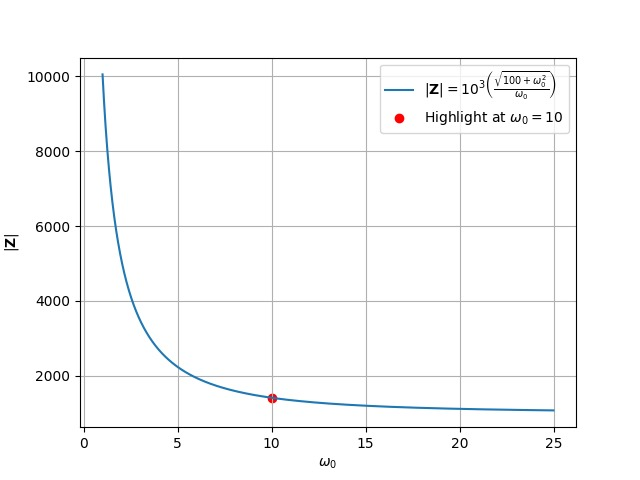
\includegraphics[width = 8cm]{2023/BM/32/figs/fig1.jpg}
		     \caption{Plot of $\abs{Z} = 10^3(\frac{\sqrt{100 + \omega_0^2}}{\omega_0}) $ }
		         \label{fig1.BM.32}
 \end{figure}
 \begin{figure}[ht]
	     \centering
	         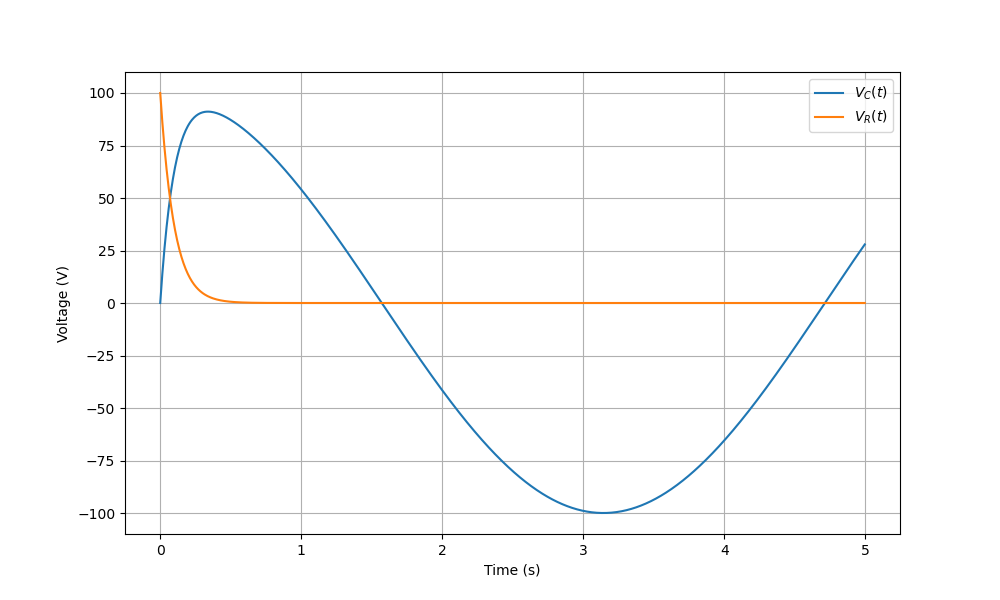
\includegraphics[width = 8cm]{2023/BM/32/figs/fig2.png}
		     \caption{Plot of Voltage Across Capacitor and Resistor}
		         \label{fig2.BM.32}
 \end{figure}
 

\pagebreak
\item Let $ w ^{4} = 16j $. Which of the fo
    llowing can not be the value of w?\\\
    \
 52 (A)   $2e^\frac{j2 \pi}{8}$\\
 53 (B)   $2e^\frac{j \pi}{8}$\\
 54 (C)   $2e^\frac{j5 \pi}{8}$\\
 55 (D)   $2e^\frac{j9 \pi}{8}$\\
\hfill{(GATE 2023 EC)}\\               \solution                              \iffalse
\let\negthickspace\undefined
\documentclass[journal,12pt,twocolumn]{IEEEtran}
\usepackage{cite}
\usepackage{amsmath,amssymb,amsfonts,amsthm}
\usepackage{algorithmic}
\usepackage{graphicx}
\usepackage{textcomp}
\usepackage{xcolor}
\usepackage{txfonts}
\usepackage{listings}
\usepackage{enumitem}
\usepackage{mathtools}
\usepackage{gensymb}
\usepackage{comment}
\usepackage[breaklinks=true]{hyperref}
\usepackage{tkz-euclide} 
\usepackage{listings}
\usepackage{gvv}                                        
\def\inputGnumericTable{}                                 
\usepackage[latin1]{inputenc}                                
\usepackage{color}                                            
\usepackage{array}                                            
\usepackage{longtable}                                       
\usepackage{calc}                                             
\usepackage{multirow}                                         
\usepackage{hhline}                                           
\usepackage{ifthen}                                           
\usepackage{lscape}
\setlength{\arrayrulewidth}{0.5mm}
\setlength{\tabcolsep}{18pt}
\renewcommand{\arraystretch}{1.5}
\newtheorem{theorem}{Theorem}[section]
\newtheorem{problem}{Problem}
\newtheorem{proposition}{Proposition}[section]
\newtheorem{lemma}{Lemma}[section]
\newtheorem{corollary}[theorem]{Corollary}
\newtheorem{example}{Example}[section]
\newtheorem{definition}[problem]{Definition}
\newcommand{\BEQA}{\begin{eqnarray}}
\newcommand{\EEQA}{\end{eqnarray}}
\newcommand{\define}{\stackrel{\triangle}{=}}
\theoremstyle{remark}
\newtheorem{rem}{Remark}
\begin{document}
\title{GATE-2023 (EC)  Q.13}
\author{EE23BTECH11051-Rajnil Malviya}
\date{February 2024}
\maketitle
\subsection*{\textit{Question :-}}
Let $ w ^{4} = 16j $. Which of the following can not be the value of w?\\\\
(A)   $2e^\frac{j2 \pi}{8}$\\
(B)   $2e^\frac{j \pi}{8}$\\
(C)   $2e^\frac{j5 \pi}{8}$\\
(D)   $2e^\frac{j9 \pi}{8}$\\
Solution:-
\fi
\begin{align}
  \brak{w^4}^{\frac{1}{4}} &= \brak{16 j}^{\frac{1}{4}}
\end{align}
Using De-Moivre's theorem for $n^{th}$ root of $w$ ,
\begin{align}
    w &=  2j^{\frac{1}{4}}\\
    e^{j\theta} &= \cos{\theta}+j\sin{\theta}\label{eq:gate23ec13rajmal}
    \end{align}
    Using equation \eqref{eq:gate23ec13rajmal} and put $\theta =\brak {2n+1} \frac{\pi}{2}$
    \begin{align}
     w &=2e^{ [j \brak {2n+1} \frac{\pi}{2}] \frac{1}{4}}
\end{align}
For different values of n ,
\begin{align}
    n&=0 \implies w =2e^{ \frac{j \pi}{8}}\\
     n&=2 \implies w =2e^{ \frac{j 5\pi}{8}}\\
      n&=4 \implies w =2e^{ \frac{j 9\pi}{8}}
\end{align}
Ans . (A) $2e^\frac{j2 \pi}{8}$
%\end{document}
     \pagebreak
\end{enumerate}
